\documentclass[3p,12pt]{article}
%\usepackage[utf8]{inputenc}
\usepackage[utf8]{vietnam}
\usepackage{amsmath, amssymb}
\usepackage{graphicx}

\title{Project 5 \\
	Taxi vận chuyển người kết hợp hàng hóa}
\author{Trần Huy Hùng \and Đỗ Ngọc Sơn}

\begin{document}
	\maketitle
		
	\section{Bài toán}
	\begin{enumerate}
		\item Cho tập các điểm:
		\begin{itemize}
			\item Điểm xuất phát $0$ của tất cả các xe taxi
			\item $N$ hành khách, hành khách $i$ có điểm đón $i$ và điểm trả $i+N+M$ ($i=1,2,...,N$)
			\item $M$ gói hàng, gói hàng $j$ ($j=N+1,N+2,...,N+M$) có:
			\begin{itemize}
				\item Điểm lấy hàng $j$ và điểm giao hàng $j+N+M$ 
				\item Khối lượng $q_j$
			\end{itemize}
			\item $d(i,j)$: Khoảng cách từ điểm $i$ đến điểm $j$ ($i,j\in \{0,1,...,2N+2M\}$)
		\end{itemize}
		\item Có $K$ xe taxi cần lập lộ trình đi từ điểm $0$, xử lý yêu cầu chuyển hành khách hoặc các gói hàng, và quay về $0$:
		\begin{itemize}
			\item Xe thứ $k$ có thể chở cùng lúc 1 hành khách và tối đa $Q_k$ khối lượng hàng ($k=1,2,...,K$)
			\item Xe đã đón khách thì phải đi thẳng đến điểm trả, không được dừng lại lấy hay giao hàng
		\end{itemize}
		\item Yêu cầu: Lập lộ trình di chuyển ngắn nhất cho các xe
	\end{enumerate}
	\begin{figure}
		\centering
		\caption{Lộ trình đón trả người kết hợp hàng hóa}
		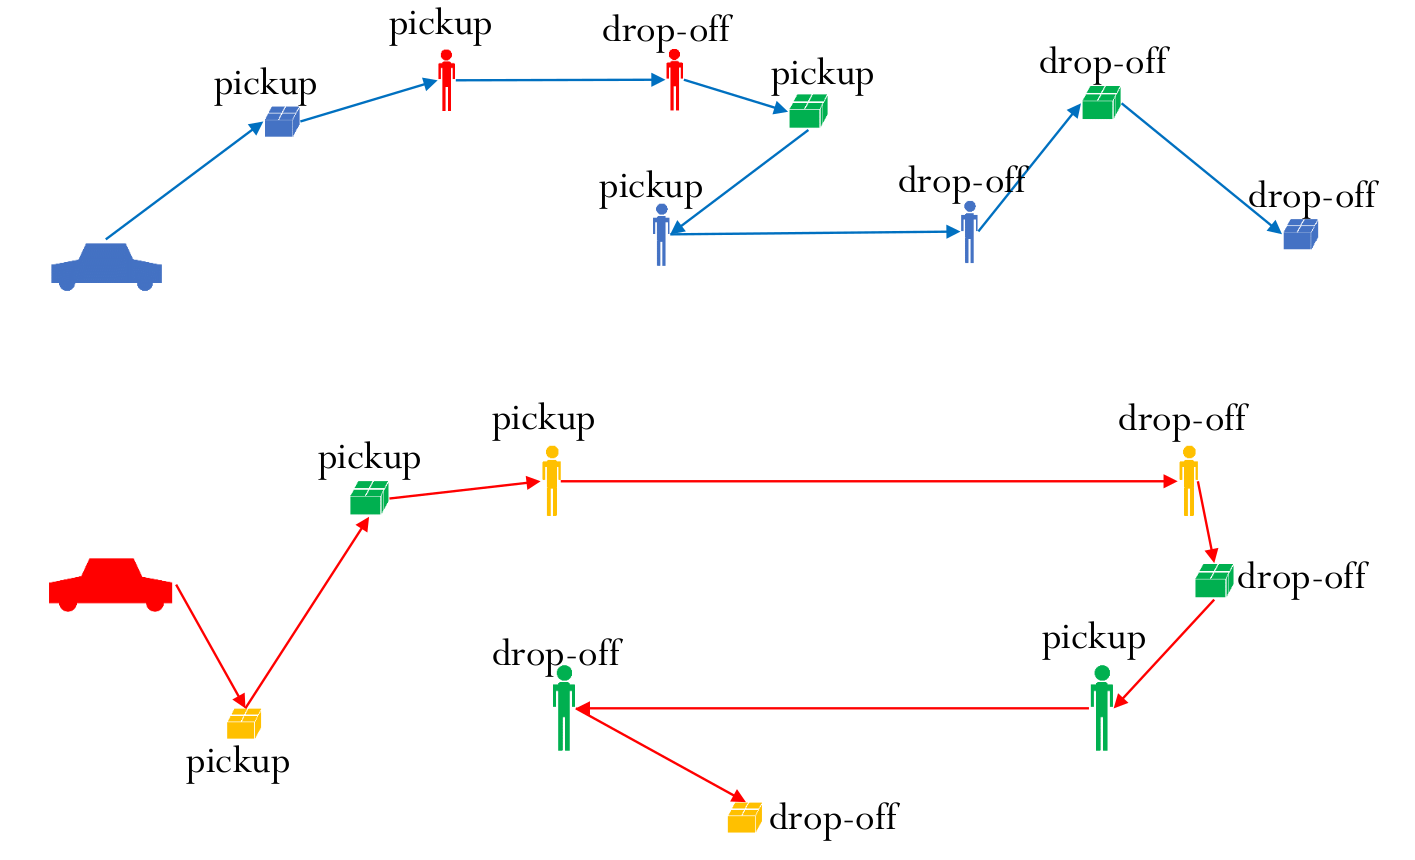
\includegraphics[width=\textwidth]{taxi.png}
	\end{figure}

	\section{Mô hình ràng buộc}
	\subsection{Tham số}
	\begin{itemize}
		\item Tập $2N+2M+K$ điểm:
		\begin{itemize}
			\item Hành khách $i$: điểm đón $i$ và điểm trả $i+N+M$ ($i=1,2,...,N$)
			\item Gói hàng $j$: điểm lấy hàng $j$ và điểm trả $j+N+M$ ($j=N+1,N+2,...,N+M$)
			\item $K$ điểm logic $2N+2M+1, 2N+2M+2, ..., 2N+2M+K$ tham chiếu tới điểm xuất phát vật lý $0$. Điểm $2N+2M+k$ tương ứng là điểm bắt đầu và kết thúc lộ trình xe thứ $k$ ($k=1,2,...,K$)
		\end{itemize}
		\item $d_{ij}$: Khoảng cách từ điểm $i$ tới điểm $j$ ($i,j\in \{1,2,...,2N+2M+K\}$)
		\item $w_i$: Sự thay đổi khối lượng hàng khi đi tới điểm $i$ ($i=1,2,...,2N+2M+K$)
		\begin{equation}
			w_i =
			\begin{cases}
			q_i & \text{nếu } N+1\leq i\leq N+M\\
			-q_{i-(N+M)} & \text{nếu } 2N+M+1\leq i\leq 2N+2M\\
			0 & \text{ngược lại}
			\end{cases} 
		\end{equation}
		\item $Q_k$: Khối lượng hàng tối đa xe thứ $k$ có thể chở ($k=1,2,...,K$)
	\end{itemize}
	\subsection{Biến quyết định}
		\begin{itemize}
			\item $x_{ij}$: Biến nhị phân, xác định cung đi từ điểm $i$ đến điểm $j$ có xuất hiện trong lộ trình của 1 trong $k$ xe không ($i,j\in \{1,2,...,2N+2M+K$)
			\begin{equation}
				x_{ij} = 
				\begin{cases}
				1 & \text{nếu cung $(i,j)$ có trong lộ trình của 1 xe}\\
				0 & \text{ngược lại}
				\end{cases}
			\end{equation}
			\item Tại mỗi điểm $i$ ($i=1,2,...,2N+2M+K$):
			\begin{itemize}
				\item $r_i$: chỉ số của xe đi qua điểm $i$ trong lộ trình
				\begin{equation}
					1\leq r_i\leq K
				\end{equation}
				\item $t_i$: thứ tự của điểm $i$ trong lộ trình của xe $k$ đi qua nó (điểm xuất phát có thứ tự 0)
				\begin{equation}
					0\leq c_i\leq 2N+2M
				\end{equation}
				\item $c_i$: khối lượng hàng xe $k$ (đi qua điểm $i$) còn chịu được khi đi tới điểm $i$
				\begin{equation}
					0\leq c_i\leq \max _{1\leq k\leq K} \{Q_k\}
				\end{equation}
			\end{itemize}
		\end{itemize}
	
	\subsection{Ràng buộc}
	\begin{itemize}
		\item Ràng buộc cân bằng luồng vào ra:
		\begin{align}
			\sum_{j=1}^{2N+2M+K} x_{ij} = 1,\quad & i=1,2,...,2N+2M+K \\
			\sum_{i=1}^{2N+2M+K} x_{ij} = 1,\quad & j=1,2,...,2N+2M+K
		\end{align}
		\item Xác định $r_i$:
		\begin{align}
			r_{2N+2M+k} = k,\quad & k=1,2,...,K \\
			x_{ij}=1\Rightarrow r_j=r_i,\quad & i=1,2,...,2N+2M+K \\
			& j=1,2,...,2N+2M \notag
		\end{align}
		\item Xác định $t_i$:
		\begin{align}
			t_{2N+2M+k} = 0,\quad & k=1,2,...,K \\
			x_{ij}=1\Rightarrow t_j=t_i + 1,\quad & i=1,2,...,2N+2M+K \\
											& j=1,2,...,2N+2M \notag
		\end{align}
		\item Xác định $c_i$:
		\begin{align}
			c_{2N+2M+k} = Q_k,\quad & k=1,2,...,K \\
			x_{ij}=1\Rightarrow c_j=c_i - w_j,\quad & i=1,2,...,2N+2M+K \\
											& j=1,2,...,2N+2M \notag
		\end{align}
		\item Điểm đón và trả của hành khách $i$ phải thuộc lộ trình của cùng một xe, tương tự với các gói hàng:
		\begin{align}
			r_i = r_{i+N+M},\quad & i=1,2,...,N+M
		\end{align}
		\item Điểm đón khách phải liền trước điểm trả khách:
		\begin{align}
			x_{i,(i+N+M)} = 1,\quad & i=1,2,...,N
		\end{align}
		\item Điểm lấy hàng phải ở trước điểm giao hàng:
		\begin{align}
			t_i < t_{i+N+M},\quad & i=N+1,N+2,...,N+M
		\end{align}
		\item Khối lượng còn lại của xe tại mọi thời điểm không âm:
		\begin{align}
			q_i \geq 0,\quad & i=1,2,...,2N+2M+K
		\end{align}
	\end{itemize}

	\subsection{Hàm mục tiêu}
	\begin{equation}
		\sum_{i=1}^{2N+2M+K} \sum_{j=1}^{2N+2M+K} d_{ij}\times x_{ij} \leftarrow min
	\end{equation}
\end{document}